\documentclass[tikz,border=8pt]{standalone}

\usepackage{amsmath,amssymb}
\usetikzlibrary{arrows.meta,backgrounds,calc,fit,positioning}

\DeclareMathOperator{\Log}{Log}

\definecolor{mlpfill}{HTML}{B7CAE8}
\definecolor{mlpdraw}{HTML}{2459A6}
\definecolor{sumfill}{HTML}{FFE2CC}
\definecolor{sumdraw}{HTML}{D95F02}
\definecolor{geomfill}{HTML}{C9C7C7}
\definecolor{geomdraw}{HTML}{4D4D4D}
\definecolor{groupdraw}{HTML}{9B9B9B}

\begin{document}
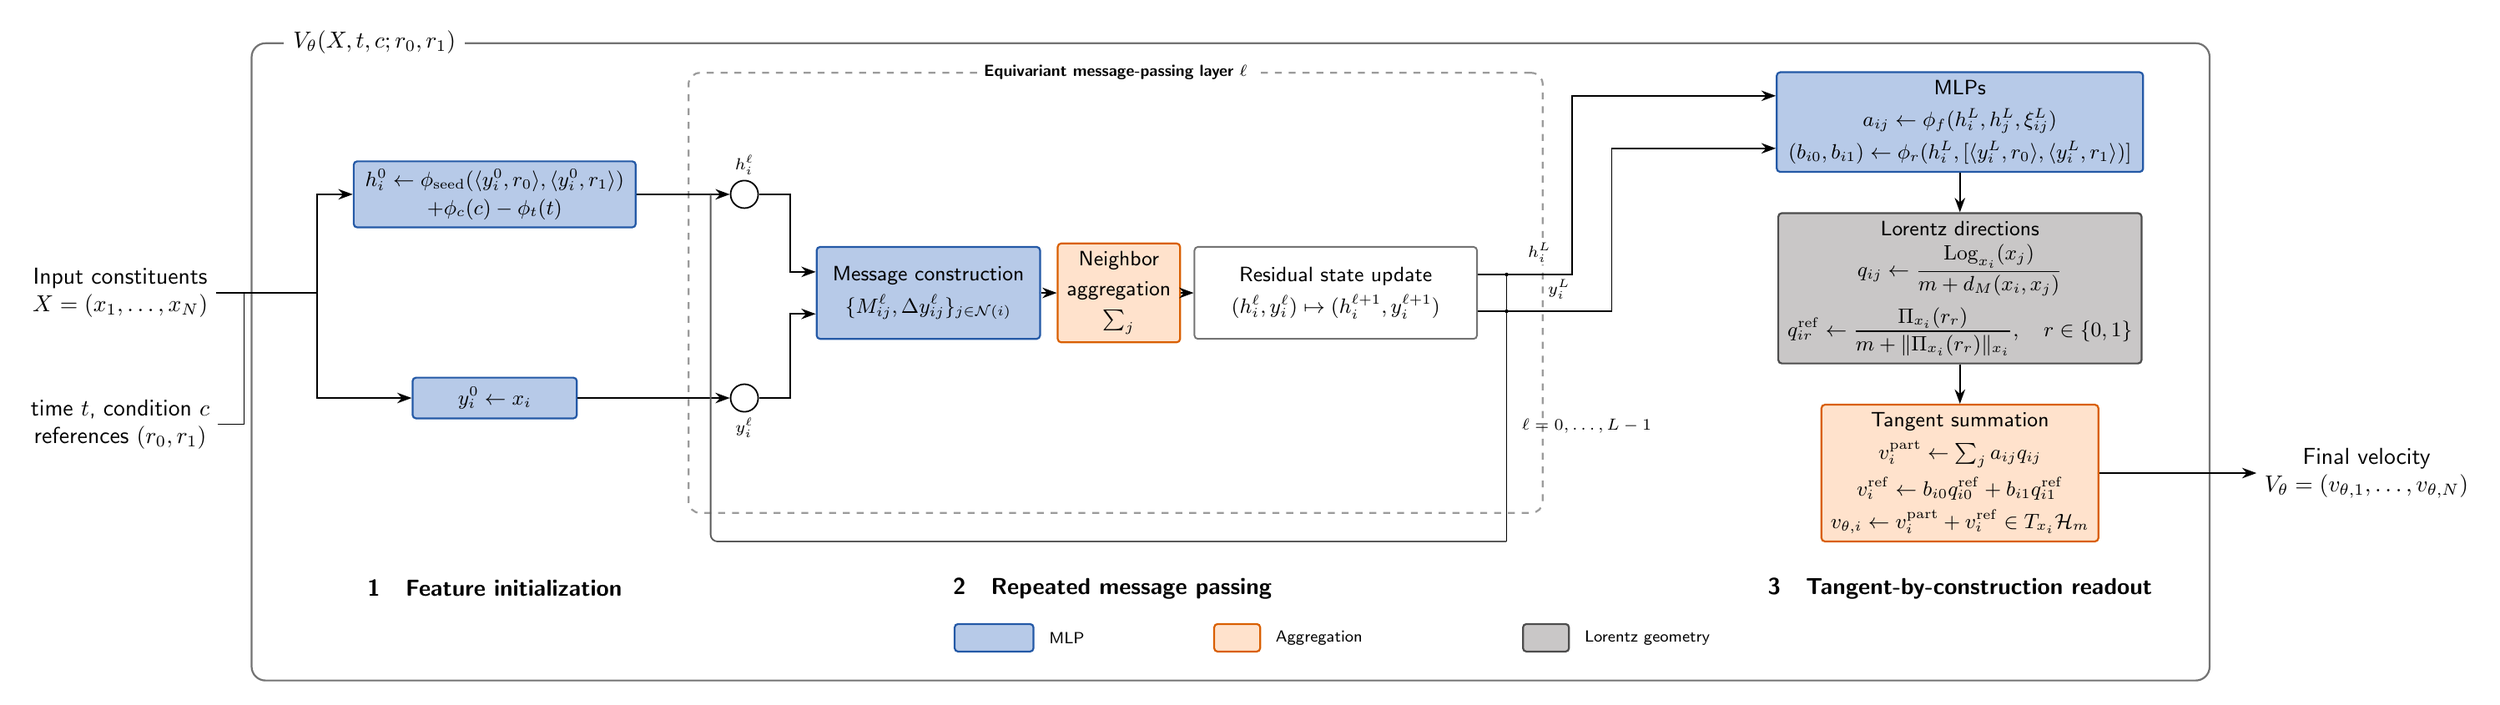
\begin{tikzpicture}[
  font=\sffamily\small,
  >={Stealth[length=2.2mm,width=1.6mm]},
  signal/.style={->, draw=black, line width=0.65pt},
  wire/.style={draw=black, line width=0.65pt},
  loop/.style={->, draw=black!65, line width=0.65pt, rounded corners=3pt},
  mlp/.style={
    draw=mlpdraw, fill=mlpfill, line width=0.8pt,
    rounded corners=1.5pt, minimum height=6.2mm,
    minimum width=25mm, align=center, inner xsep=5pt
  },
  sum/.style={
    draw=sumdraw, fill=sumfill, line width=0.8pt,
    rounded corners=1.5pt, minimum height=5.6mm,
    minimum width=18mm, align=center, inner xsep=4pt
  },
  geometry/.style={
    draw=geomdraw, fill=geomfill, line width=0.8pt,
    rounded corners=1.5pt, minimum height=5.6mm,
    minimum width=18mm, align=center, inner xsep=4pt
  },
  result/.style={
    draw=black!55, fill=white, line width=0.7pt,
    rounded corners=1.5pt, minimum height=5.8mm,
    minimum width=20mm, align=center, inner xsep=5pt
  },
  junction/.style={
    circle, draw=black, fill=white, line width=0.65pt,
    minimum size=4.2mm, inner sep=0pt, font=\scriptsize
  },
  stage title/.style={font=\sffamily\bfseries, align=center},
  annotation/.style={font=\sffamily\scriptsize, align=center},
  io/.style={font=\sffamily, align=center}
]

% =============================================================================
% STAGE 1: Feature Initialization
% =============================================================================
\node[mlp] (seedH) at (-1.8,1.5)
  {$h_i^0\leftarrow\phi_{\rm seed}(\langle y_i^0,r_0\rangle,
    \langle y_i^0,r_1\rangle)$\\[1pt]
   $+\phi_c(c)-\phi_t(t)$};
\node[mlp] (seedY) at (-1.8,-1.6) {$y_i^0\leftarrow x_i$};
\node[stage title] at (-1.8,-4.5)
  {1\quad Feature initialization};

% =============================================================================
% STAGE 2: Compact Repeated Message-Passing Stack
% =============================================================================
\node[junction] (jH) at (2,1.5) {};
\node[junction] (jY) at (2,-1.6) {};
\node[annotation, above=5pt] at (jH) {$h_i^\ell$};
\node[annotation, below=5pt] at (jY) {$y_i^\ell$};

\node[mlp, minimum width=34mm, minimum height=14mm]
  (messageSummary) at (4.8,0)
  {Message construction\\[3pt]
   $\{M_{ij}^\ell,\Delta y_{ij}^\ell\}_{j\in\mathcal N(i)}$};
\node[sum, minimum width=17mm, minimum height=14mm]
  (sumSummary) at (7.7,0)
  {Neighbor\\[2pt]aggregation\\[2pt]$\sum_j$};
\node[result, minimum width=43mm, minimum height=14mm]
  (updateSummary) at (11.0,0)
  {Residual state update\\[3pt]
   $(h_i^\ell,y_i^\ell)\mapsto
    (h_i^{\ell+1},y_i^{\ell+1})$};

\draw[signal] (seedH.east) -- (jH);
\draw[signal] (seedY.east) -- (jY);
\draw[signal] (jH) -- ++(0.7,0)
  |- ($(messageSummary.west)+(0,0.32)$);
\draw[signal] (jY) -- ++(0.7,0)
  |- ($(messageSummary.west)+(0,-0.32)$);
\draw[signal] (messageSummary.east) -- (sumSummary.west);
\draw[signal] (sumSummary.east) -- (updateSummary.west);

% Two updated states leave on short horizontal branches.  Their shared
% vertical spine is used only for the recurrent application of the layer.
\coordinate (feedbackAxis) at (13.6,0);
\coordinate (hFork) at (13.6,0.28);
\coordinate (yFork) at (13.6,-0.28);
\draw[wire] ($(updateSummary.east)+(0,0.28)$) -- (hFork);
\draw[wire] ($(updateSummary.east)+(0,-0.28)$) -- (yFork);
\draw[wire] (hFork) -- (yFork);
\fill (hFork) circle[radius=0.8pt];
\fill (yFork) circle[radius=0.8pt];

% Compact layer boundary and recurrent application.
\coordinate (layerNW) at (1.35,3.15);
\coordinate (layerSE) at (13.95,-3.15);
\begin{scope}[on background layer]
  \node[
    draw=groupdraw, dashed, line width=0.8pt, rounded corners=5pt,
    fit=(layerNW)(layerSE)(jH)(jY)(messageSummary)(sumSummary)(updateSummary),
    inner xsep=2mm, inner ysep=2mm
  ] (layerGroup) {};
\end{scope}
\node[annotation, font=\sffamily\scriptsize\bfseries,
      fill=white, inner xsep=3pt]
  at (layerGroup.north)
  {Equivariant message-passing layer $\ell$};

\coordinate (feedbackJoin) at
  ($(feedbackAxis |- layerGroup.south)+(0,-0.42)$);
\draw[wire] (yFork)
  -- node[annotation, midway, right=3pt] {$\ell=0,\ldots,L-1$}
     (feedbackJoin);
\coordinate (returnCorner) at
  ($(layerGroup.south west)+(0.35,-0.42)$);
\coordinate (returnTop) at
  (returnCorner |- jH);
\draw[wire, draw=black!65, rounded corners=3pt]
  (feedbackJoin) -- (returnCorner) -- (returnTop);


\node[stage title] at (7.6,-4.5)
  {2\quad Repeated message passing};

% =============================================================================
% STAGE 3: Tangent-by-Construction Readout
% =============================================================================
\node[mlp] (readoutMlp) at (20.5,2.6)
  {MLPs\\[3pt]
   $a_{ij}\leftarrow\phi_f(h_i^L,h_j^L,\xi_{ij}^L)$\\[3pt]
   $(b_{i0},b_{i1})\leftarrow
    \phi_r(h_i^L,[\langle y_i^L,r_0\rangle,\langle y_i^L,r_1\rangle)]$};
\node[geometry, below=6mm of readoutMlp] (directions)
  {Lorentz directions\\[3pt]
   $q_{ij}\leftarrow\dfrac{\Log_{x_i}(x_j)}{m+d_M(x_i,x_j)}$\\[4pt]
   $q_{ir}^{\rm ref}\leftarrow
    \dfrac{\Pi_{x_i}(r_r)}{m+\|\Pi_{x_i}(r_r)\|_{x_i}},
    \quad r\in\{0,1\}$};
\node[sum, below=6mm of directions] (signedSum)
  {Tangent summation\\[3pt]
   $v_i^{\rm part}\leftarrow\sum_j a_{ij}q_{ij}$\\[3pt]
   $v_i^{\rm ref}\leftarrow b_{i0}q_{i0}^{\rm ref}
      +b_{i1}q_{i1}^{\rm ref}$\\[3pt]
   $v_{\theta,i}\leftarrow v_i^{\rm part}+v_i^{\rm ref}
      \in T_{x_i}\mathcal H_m$};

\draw[signal] (hFork) -- ++(1.0,0)
  node[annotation, midway, above=4pt, fill=white, inner sep=1pt] {$h_i^L$}
  |- ($(readoutMlp.west)+(0,0.4)$);
\draw[signal] (yFork) -- ++(1.6,0)
  node[annotation, midway, above=4pt, fill=white, inner sep=1pt] {$y_i^L$}
  |- ($(readoutMlp.west)+(0,-0.4)$);
\draw[signal] (readoutMlp.south) -- (directions.north);
\draw[signal] (directions.south) -- (signedSum.north);
\node[stage title] at (20.5,-4.5)
  {3\quad Tangent-by-construction readout};

% =============================================================================
% Model Boundary, External Inputs, and Final Velocity
% =============================================================================
\coordinate (modelNW) at (-5.5,3.8);
\coordinate (modelSE) at (24.3,-5.9);
\begin{scope}[on background layer]
  \node[
    draw=black!55, line width=0.8pt, rounded corners=6pt,
    fit=(modelNW)(modelSE), inner sep=0pt
  ] (model) {};
\end{scope}
\node[font=\sffamily\bfseries, fill=white,
      inner xsep=4pt, anchor=west]
  at ($(model.north west)+(0.5,0)$)
  {$V_\theta(X,t,c;r_0,r_1)$};

\node[io] (inputX) at (-7.5,0)
  {Input constituents\\$X=(x_1,\ldots,x_N)$};
\node[io] (inputC) at (-7.5,-2.0)
  {time $t$, condition $c$\\references $(r_0,r_1)$};
\draw[wire] (inputC.east) -- ++(0.4,0) coordinate (bracketC);
\draw[wire] (bracketC) |- (inputX.east);
\coordinate (splitX) at (-4.5,0);
\draw[wire] (inputX.east) -- (splitX);
\draw[signal] (splitX) |- (seedH.west);
\draw[signal] (splitX) |- (seedY.west);

\node[io, anchor=west] (output)
  at ($(model.east |- signedSum.east)+(0.7,0)$)
  {Final velocity\\$V_\theta=(v_{\theta,1},\ldots,v_{\theta,N})$};
\draw[signal] (signedSum.east) -- (output.west);

% Operation legend.
\node[mlp, minimum width=12mm, minimum height=4.2mm]
  (legendMlp) at (5.8,-5.25) {};
\node[annotation, right=1mm of legendMlp] {MLP};
\node[sum, minimum width=7mm, minimum height=4.2mm]
  (legendSum) at (9.5,-5.25) {};
\node[annotation, right=1mm of legendSum] {Aggregation};
\node[geometry, minimum width=7mm, minimum height=4.2mm]
  (legendGeom) at (14.2,-5.25) {};
\node[annotation, right=1mm of legendGeom] {Lorentz geometry};

\end{tikzpicture}
\end{document}
